%============================================================
% SASA R&E 보고서 양식 (2026) — main.tex
%
% ── Overleaf 사용 시 최초 1회 설정 ──────────────────────────
%  화면 왼쪽 위 Menu(≡) 클릭 후 아래와 같이 설정하세요.
%
%   Compiler     →  XeLaTeX      (기본값인 pdfLaTeX은 한글 불가)
%   Bibliography →  Biber        (기본값인 BibTeX은 참고문헌 오류)
%
%  설정 후 Recompile 버튼을 누르면 됩니다.
% ────────────────────────────────────────────────────────────
%
% ── 편집 순서 안내 ───────────────────────────────────────────
%  1. 00_info.tex      — 제목·저자·날짜 등 기본 정보 입력
%  2. 03_summaries.tex — 1·2페이지 요약문 표 내용 작성
%  3. 01_abstract.tex  — 국문 초록 작성 (논문 완성 후 마지막에)
%  4. 02_body.tex      — 본문 작성
%  5. refs.bib         — 참고문헌 추가
%
%  이 파일(main.tex)과 나머지 파일은 수정하지 않아도 됩니다.
%============================================================

\documentclass[10pt]{oblivoir}

%============================================================
% 00_info.tex — 논문 기본 정보
% 이 파일만 편집하면 표지·별첨·3페이지 제목에 자동으로 반영됩니다.
%============================================================

\def\mytitleko{우리말 제목}   % 논문 국문 제목
\def\mytitle{English Title}   % 논문 영문 제목

\def\myauthorfirstko{홍길동1}          % 저자1 국문 이름
\def\myauthorsecondko{홍길동2}         % 저자2 국문 이름
\def\myauthorfirst{Hong Gildong1}      % 저자1 영문 이름 (성 Gildong, 이름 Hong 순서 주의)
\def\myauthorsecond{Hong Gildong2}     % 저자2 영문 이름

\def\affiliationko{세종과학예술영재학교}
\def\affiliation{Sejong Academy of Science and Arts}
\def\address{265, Dalbit 1-ro, Sejong-si, Republic of Korea}

\def\mykeywordsko{주요어1, 주요어2, 주요어3}   % 국문 주요어 (쉼표로 구분, 5개 이내)
\def\mykeywords{keyword1, keyword2, keyword3}   % 영문 키워드

\def\mydate{2026년\quad 11월\quad OO일}   % 제출일 (\quad는 공백, OO을 날짜로 교체)
\def\myadvisor{OOO}                        % 지도교사 이름
     % 논문 메타데이터
% RnE 보고서 양식 스타일 파일
% 패키지·환경·명령어 설정만 — 본문 내용 없음

%-- 용지 설정
\usepackage{fapapersize}
\usefastocksize{210mm,297mm}
\usefapapersize{210mm,297mm,25mm,25mm,25mm,25mm}

%-- 수식
\usepackage{mathtools}
\usepackage{amsthm}
\usepackage{amssymb}
\usepackage{mathrsfs}

%-- 그래픽
\usepackage{graphicx}
\usepackage{xcolor}

%-- 텍스트·레이아웃
\usepackage{setspace}
\usepackage{lipsum}
\usepackage{jiwonlipsum}
\usepackage{ragged2e}
\usepackage{textpos}
\usepackage{kskorsymb}

%-- 표
\usepackage{tabularray}
\UseTblrLibrary{booktabs}
\newlength\mycellwidth  % 셀 병합에서 사용하는 길이 변수

%-- 캡션
\usepackage{caption}
\DeclareCaptionLabelFormat{cjk-single-bracket}{[#1 #2]}
\captionsetup[figure]{labelsep=space, labelfont=bf,
  labelformat=cjk-single-bracket, name={Fig.}}
\captionsetup[table]{labelsep=period, labelfont=bf, name={Table}}

%-- 섹션 번호 형식
\renewcommand\thesection{\Roman{section}}
\renewcommand\thesubsection{\arabic{subsection}}
\renewcommand\thesubsubsection{\thesubsection.\arabic{subsubsection}}
\setsecnumformat{\csname the#1\endcsname.\ }
\setcounter{secnumdepth}{3}
\renewcommand{\abstractname}{Abstract}

%-- 정리류 환경
\newtheorem{theorem}{\bfseries\sffamily 정리}
\newtheorem{lemma}[theorem]{도움정리}
\newtheorem{corollary}[theorem]{따름정리}
\theoremstyle{definition}
\newtheorem{definition}[theorem]{정의}
\newtheorem{example}[theorem]{보기}
\theoremstyle{remark}
\newtheorem{remark}[theorem]{참고}
\numberwithin{equation}{section}
\renewcommand*{\proofname}{증명}

\allowdisplaybreaks

%-- 커스텀 명령어
% 수식 안 쉼표에서 줄바꿈 허용
\newcommand{\splitatcommas}[1]{%
  \begingroup
  \begingroup\lccode`~=`, \lowercase{\endgroup
    \edef~{\mathchar\the\mathcode`, \penalty0 \noexpand\hspace{0pt plus 1em}}%
  }\mathcode`,="8000 #1%
  \endgroup
}

% 체크된 체크박스
\newcommand{\mycheckedbox}{$\square$\!\!\!\!\checkmark}

% 각 페이지 상단 헤더 (1·2·3페이지 섹션 제목)
% 선택 인수: 헤더 아래 수직 여백 (기본 23pt)
\newcommand{\RnEpageheader}[2][23pt]{%
  \begin{textblock*}{\textwidth}(0cm,0cm)%
    \noindent\LARGE\bfseries #2%
  \end{textblock*}%
  \vspace{#1}%
}

%-- 참고문헌 설정
% 참고문헌 설정 (biblatex + biber)

\usepackage[backend=biber, natbib=true, sorting=none,
  citestyle=numeric-comp, bibstyle=numeric,
  maxbibnames=10, minbibnames=6,
  maxcitenames=6, mincitenames=1]{biblatex}
\addbibresource{refs.bib}

\renewbibmacro{in:}{}
\DeclareFieldFormat[article]{volume}{\emph{#1}}
\DeclareFieldFormat{pages}{#1}
\renewcommand{\finalnamedelim}{\ \&\ }

\renewbibmacro*{volume+number+eid}{%
  \printfield{volume}%
  \printfield{number}%
  \setunit{\addcomma\space}%
  \printfield{eid}}
\DeclareFieldFormat[article]{number}{\mkbibparens{#1}}

\AtEveryBibitem{%
  \DeclareFieldFormat[article,inproceedings]{title}{#1}%
  \ifkeyword{kobib}{%
    \renewcommand{\multinamedelim}{, }%
    \renewcommand{\finalnamedelim}{, }%
    \DeclareFieldFormat[article]{volume}{\textbf{#1}}%
    \DeclareFieldFormat*{journaltitle}{#1,}%
    \DeclareFieldFormat*{titlecase}{%
      \ifdef{\currentfield}
        {\ifcurrentfield{journaltitle}
           {\usefield{\textbf}{\currentfield}}%
           {#1}}
        {#1}}%
    \DeclareFieldFormat*[book,thesis]{title}{#1}%
    \DeclareFieldFormat*[book,thesis]{titlecase}{%
      \ifdef{\currentfield}
        {\ifcurrentfield{title}
           {\usefield{\textbf}{\currentfield}}%
           {#1}}
        {#1}}%
  }{}%
}

\AtEveryCitekey{%
  \ifkeyword{kobib}{%
    \renewcommand{\multinamedelim}{, }%
    \renewcommand{\finalnamedelim}{, }%
  }{}%
}

\DefineBibliographyStrings{english}{phdthesis = {박사학위논문}}
\DefineBibliographyStrings{english}{mathesis  = {석사학위논문}}

\newbibmacro*{institution+thesistype+location+date}{%
  \printlist{location}%
  \iflistundef{institution}
    {\setunit*{\addcomma\space}}
    {\setunit*{\addcolon\space}}%
  \printlist{institution}%
  \setunit*{\addspace}%
  \printfield{type}%
  \setunit*{\addcomma\space}%
  \usebibmacro{date}%
  \newunit}

\usepackage{xpatch}
\xpatchbibdriver{thesis}
  {\printfield{type}%
   \newunit
   \usebibmacro{institution+location+date}}
  {\usebibmacro{institution+thesistype+location+date}}
  {}{}

\DeclareDelimFormat[textcite]{nameyeardelim}{}


%-- 요약문 매크로 (학생 편집: 03_summaries.tex)
%============================================================
% 03_summaries.tex — 1·2페이지 표 내용
%
% 이 파일의 각 \newcommand가 다음 칸을 채웁니다.
%   1페이지(연구결과 요약문): summaryGoal / summaryResult / summaryEffect
%   2페이지(과제 수행 과정): summaryExpert / summaryProblemSolving /
%                            summaryFirstMember / summarySecondMember / summaryLearning
%
% \jiwon[숫자]는 한글 더미 텍스트입니다 (Lorem ipsum의 한글 버전).
% 각 칸의 \jiwon[...] 줄을 지우고 실제 내용을 작성하세요.
% 여러 문단을 써도 되고, 줄바꿈도 사용할 수 있습니다.
%============================================================

%%% 1페이지 ─────────────────────────────────────────────────

\newcommand{\summaryGoal}{%
  % '연구 필요성 및 목적' 칸
  \jiwon[1] % ← 이 줄을 지우고 내용을 작성하세요
}

\newcommand{\summaryResult}{%
  % '연구내용 및 연구결과' 칸
  \jiwon[2-3] % ← 이 줄을 지우고 내용을 작성하세요
}

\newcommand{\summaryEffect}{%
  % '연구 기대효과' 칸
  \jiwon[4] % ← 이 줄을 지우고 내용을 작성하세요
}

%%% 2페이지 ─────────────────────────────────────────────────

\newcommand{\summaryExpert}{%
  % '전문가 피드백 활용 과정' 칸
  % 전문가 피드백을 받지 않았다면 아래 한 줄로 대체하세요.
  %   해 당 없 음
  \jiwon[5] % ← 이 줄을 지우고 내용을 작성하세요
}

\newcommand{\summaryProblemSolving}{%
  % '문제해결 과정' 칸 — 팀 전체의 과정을 서술
  \jiwon[6-7] % ← 이 줄을 지우고 내용을 작성하세요
}

\newcommand{\summaryFirstMember}{%
  % '팀원1' 칸 — 00_info.tex의 \myauthorfirstko(저자1)의 역할
  \jiwon[8] % ← 이 줄을 지우고 내용을 작성하세요
}

\newcommand{\summarySecondMember}{%
  % '팀원2' 칸 — 00_info.tex의 \myauthorsecondko(저자2)의 역할
  \jiwon[8] % ← 이 줄을 지우고 내용을 작성하세요
}

\newcommand{\summaryLearning}{%
  % '과제 수행 과정에서의 학습' 칸
  \jiwon[9] % ← 이 줄을 지우고 내용을 작성하세요
}

   % 패키지·환경 설정

% 필요한 경우 아래 주석을 해제하세요:
% \usepackage{tikz}         % TikZ 그림
% \usepackage{mathrsfs}     % \mathscr 글꼴

\begin{document}

\pagestyle{empty}

%%% 1페이지: 연구결과 요약문
\RnEpageheader{1. 연구결과 요약문}
\begin{center}
  \begin{tblr}{
      width = \textwidth,
      colspec = {Q[1,c,m,gray!20]Q[3.88,m]},
      hlines,
      vline{1-Z} = {solid},
      column{1} = {font=\bfseries\sffamily},
    }
    과 제 명                    & \mytitleko      \\
    {연구 필요성\\ 및 목적}       & \summaryGoal    \\
    {연구내용 \\ 및 \\ 연구결과}  & \summaryResult  \\
    연구 기대효과                 & \summaryEffect  \\
    {Keyword\\ (5개 이내)}       & \mykeywordsko   \\
  \end{tblr}
\end{center}

\newpage

%%% 2페이지: 과제 수행 과정
\RnEpageheader{2. 과제 수행 과정}
\begin{center}
  \setlength\mycellwidth{\dimexpr\linewidth - \parindent - 2.5cm - 2.5em\relax}
  \begin{tblr}{
      width = \textwidth,
      colspec = {Q[2.5cm,c,m,gray!20]X[.7,m]X[4.96,m]},
      hlines,
      vline{1-Z} = {solid},
      column{1} = {font=\bfseries\sffamily},
    }
    {전문가 \\ 피드백 활용 \\ 과정}
      & \SetCell[c=2]{c} \parbox{\mycellwidth}{\justifying\summaryExpert} & \\
    \SetCell[r=3]{c,m} {문제해결 \\ 과정}
      & \SetCell[c=2]{m} \parbox{\mycellwidth}{\justifying\summaryProblemSolving} & \\
      & \SetCell{l,t} 팀원1 & \summaryFirstMember \\
      & \SetCell{l,t} 팀원2 & \summarySecondMember \\
    {과제 수행 \\ 과정에서의 \\ 학습}
      & \SetCell[c=2]{c} \parbox{\mycellwidth}{\justifying\summaryLearning} & \\
  \end{tblr}
\end{center}

\newpage

%%% 3페이지: 논문 제목 표시 (연구결과 시작)
\RnEpageheader[18pt]{3. 연구결과}
\begin{center}
  \begin{spacing}{1.3}
    {\LARGE\bfseries \mytitleko}\par
    \vspace{5pt}
    \textcolor{gray}{\myauthorfirstko, \myauthorsecondko}\par
    \textcolor{gray}{\affiliationko}
  \end{spacing}
  \vspace{10pt}
  {\large\bfseries \mytitle}\par
  \vspace{5pt}
  \textcolor{gray}{\myauthorfirst, \myauthorsecond}\par
  \textcolor{gray}{\affiliation}
\end{center}

%============================================================
% 01_abstract.tex — 국문 초록
%
% 초록은 논문 전체를 한 단락으로 요약한 글입니다.
% 연구 목적 · 방법 · 결과 · 결론의 흐름으로 작성하며,
% 분량은 보통 200~400자 내외입니다.
% 논문을 다 쓴 뒤 마지막에 작성하는 것을 권장합니다.
%============================================================

\begin{center}
  {\Large\textbf{국문 초록}}
  \noindent\rule{\textwidth}{.12mm}
\end{center}

초록은 언제 쓰는가? 맨 나중에 쓰는게 국룰이다. 진짜? 당연하지. 초록은 논문의 얼굴과 같다. 선행연구 \citep{smith1987tiling}에 의하면 어쩌고 저쩌고.
% ↑ 위 예시 문장을 지우고 실제 초록을 작성하세요.
% 본문에서 인용한 참고문헌은 초록에서도 \citep{키} 형식으로 표기할 수 있습니다.

\vskip5pt
\noindent{\bfseries 주제어:}\ \mykeywordsko
% 주제어는 00_info.tex의 \mykeywordsko에서 자동으로 가져옵니다.

\noindent\rule{\textwidth}{.12mm}


%============================================================
% 02_body.tex — 본문
%
% 이 파일에 논문 본문을 작성합니다.
% 아래 내용은 사용 방법을 안내하는 예시이므로,
% 내용을 확인한 뒤 지우고 실제 논문을 작성하세요.
%
% 섹션 구조:
%   \section{제목}           → I. 제목  (로마 숫자 자동)
%   \subsection{제목}        → 1. 제목
%   \subsubsection{제목}     → 1.1. 제목
%============================================================


%------------------------------------------------------------
\section{서론}
%------------------------------------------------------------

\jiwon[2]
% \jiwon[숫자]는 한글 더미 텍스트입니다 (Lorem ipsum의 한글 버전).
% 위 줄을 지우고 서론을 작성하세요.


%------------------------------------------------------------
\section{이론적 배경 및 선행연구 조사}\label{sec:search}
%------------------------------------------------------------
% \label{이름}을 붙이면 본문 어디서든 \ref{이름}으로 해당 번호를 참조할 수 있습니다.

\subsection{소제목}
\subsubsection{과학영재 창의연구(R\&E)}
% R\&E 처럼 특수문자 &는 앞에 \를 붙여야 합니다.

\jiwon[6-7]

앞서 \ref{sec:search}절에서 본 바와 같이 이론적 배경은 매우 어렵다.
% \ref{sec:search}는 위의 \label{sec:search}가 붙은 절 번호를 자동으로 가져옵니다.


%------------------------------------------------------------
% [그림 삽입 예시]
% images/ 폴더에 그림 파일을 넣은 뒤 아래와 같이 삽입합니다.
%------------------------------------------------------------

\begin{figure}[!ht]
  \centering
  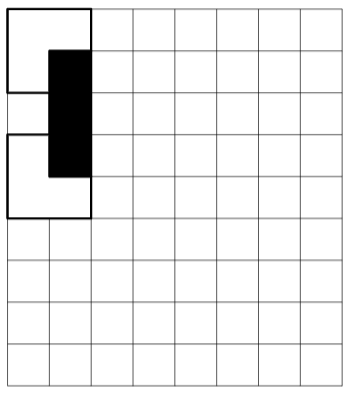
\includegraphics[width=.15\textwidth]{images/B(8, 9).png}
  % width=.15\textwidth → 텍스트 폭의 15%. 크기를 자유롭게 조절하세요.
  \caption{bad pair of $9\times 8$ deficient tile}
  % \caption{} 안에 그림 설명을 씁니다.
  \label{fig:my_label}
  % \label{}로 이름을 붙이면 본문에서 그림 \ref{fig:my_label}로 참조할 수 있습니다.
\end{figure}


%------------------------------------------------------------
% [정리류 환경 예시]
% 사용 가능한 환경: theorem(정리), lemma(보조정리), corollary(따름정리),
%                   definition(정의), example(보기), remark(참고)
%------------------------------------------------------------

\begin{definition}
  정의란 무엇일까? \citep{aanjaneya2009tromino, golomb2021polyominoes, nitica2017tilings}
  % \citep{키}로 참고문헌을 인용합니다. 키는 refs.bib 파일에 정의되어 있습니다.
  % 여러 문헌을 동시에 인용할 때는 쉼표로 구분합니다.
\end{definition}

\jiwon[3-4]

\begin{theorem}\label{thm:what}
  정리란 무엇일까?
\end{theorem}


%------------------------------------------------------------
\subsection{그림 삽입 방법}
%------------------------------------------------------------

아래에서는 그림을 삽입하는 방법을 안내한다. 크게 두 가지 방법이 있다.
\begin{enumerate}[(a)]
  \item 그림 파일을 images 폴더에 업로드 한 후, 그 파일을 넣는 방식.
  \item 텍을 이용하여 직접 그림을 그리는 방식.
\end{enumerate}
그러나, 어느 방식이든, 그림의 위치를 \TeX에게 맡기려면, figure 환경을 이용해야한다.
또 하나의 팁을 주자면, 그림파일을 미리 준비하지 않았더라도, \TeX이 갖고 있는 예시그림을 이용하여
그림의 위치를 미리 어느 정도 살펴볼 수 있다는 것이다.

다음 예시는 \TeX이 갖고 있는 그림예제를 이용하여 그림을 삽입해 본 것이다.

\begin{figure}[!ht]
  \centering
  \includegraphics[width=.4\textwidth]{example-image}
  % example-image는 TeX이 기본 제공하는 예시 그림입니다.
  % 실제 사용할 때는 images/파일명.png 처럼 직접 준비한 파일로 교체하세요.
  \caption{이 그림의 캡션은?!}
  \label{fig:my_fig_label}
\end{figure}

figure 환경에 넣은 그림에는 각 그림에 label을 지정해두었으므로, 상호참조 기능을 이용하여
``그림 \ref{fig:my_label}\을 참고하라.''와 같이 해당 그림을 언급할 수 있다.

한가지 유의할 점은, 논문에서 그림은 필요한 경우에만 넣는다는 것이다. 다시 말해, 논문에
그림을 넣는 것은 논문의 내용에 (상호참조 등을 통해) 그 그림이 언급될 때만 가능한 것으로
여기는 것이 일반적이다. 따라서 논문에 등장하는 모든 그림은 figure 환경에 넣는 것이 바람직하다 하겠다.


%------------------------------------------------------------
\subsection{표 삽입 방법}
%------------------------------------------------------------

한편 표를 삽입하는 방법은 그림을 삽입하는 방법과 거의 동일하다. figure 환경을 table환경으로
바꾸기만 하면 된다.

\begin{table}[!ht]
  \centering
  \caption{이 표의 캡션은?!}
  % 표의 캡션은 표 위에 옵니다 (\caption을 \begin{tblr} 앞에 두세요).
  \label{tab:my_label}
  \begin{tblr}{hlines, vlines}
    % hlines: 가로선, vlines: 세로선 모두 표시
         & 위치 & 장소 \\
    1    &      &      \\
    2    &      &      \\
    3    &      &      \\
  \end{tblr}
\end{table}

한편 표 \ref{tab:my_booktablabel}에서 볼 수 있는 표 양식은 여러 타이포그라피 교과서에서
권장하는 양식이며, 서구권에서 표준적으로 사용하는 양식이라 할 수 있다.
\begin{table}[!ht]
  \centering
  \caption{예쁜 표의 캡션은?!}
  \label{tab:my_booktablabel}
  \begin{booktabs}{colspec={cccc}}
    % booktabs 환경은 가로선만 있는 깔끔한 표를 만듭니다.
    \toprule
    Case & Box A & Box B & Remarks \\
    \midrule
    \SetCell[r=2]{c,m} A & $+X$ & $-1.0$ & \SetCell[r=2]{c,m} B \\
    \cmidrule[lr]{2-3}
    & $-X$ & $-7.9$ & \\
    \bottomrule
  \end{booktabs}
\end{table}


%------------------------------------------------------------
\subsection{수식 입력 방법}
%------------------------------------------------------------

이번에는 수식을 작성하는 몇 가지 예를 살펴보자. 수식은 크게 두 가지 모드로 작성한다.
\begin{itemize}
  \item 행중수식: 문단 안에 $처럼$ 달러 기호로 감싸 쓰는 수식 \quad 예: $E = mc^2$
  \item 행간수식: 별도의 줄에 \verb|\[ ... \]|로 감싸 쓰는 수식
\end{itemize}

\begin{itemize}
  \item 아래첨자: $A_{b+c}$ (cf. $A_a+b$). 곱하기는 $a\times b$.

  \item 최대정수함수 — \verb|\left|·\verb|\right|로 괄호 크기를 내용에 맞게 조절합니다.
    \[ \left\lfloor \frac{\pi^2}{6}\right\rfloor \]

  \item 분수: $\frac{2}{3}$ \quad 행간수식에서는 분수가 크게 표시됩니다.
    \[ \frac{df}{dt}=\frac{df}{ds}\frac{ds}{dt} \]

  \item 부등호: $1\leq 3\leq 5 \geq 2$.

  \item 여러 줄 정렬 수식 — \verb|&|는 정렬 기준, \verb|\\|은 줄바꿈입니다.
    \begin{align*}
      a & \equiv b \mod{p} \\
      a & \equiv b \pmod{p}
    \end{align*}
\end{itemize}


%------------------------------------------------------------
\section{결론}
%------------------------------------------------------------

\jiwon[4]
% ↑ 지우고 결론을 작성하세요.


\section{참고문헌}
\printbibliography[heading=none]
% \nocite{key}  % 본문에서 인용하지 않았지만 목록에 넣을 항목

\newpage
%%% 별첨 (수정하지 마세요) %%%

%%% 별첨 1: 연구윤리 체크리스트 (학생용)
\defineextraparenmark{【 】}
\begin{textblock*}{\textwidth}(0cm,0cm)
  \noindent "/별첨 1"/
\end{textblock*}
\vspace{15pt}

\begin{center}
  {\LARGE\bfseries 연구윤리 체크리스트}{\large\bfseries (학생용)}
  \vspace{15pt}

  \begin{tblr}{
      width = \textwidth,
      colspec = {Q[2.5cm,c,m]X[3.625,m]X[.575,c]X[.575,c]},
      hlines,
      rowsep = 5pt,
      vline{1-Z} = {solid},
      column{1} = {font=\bfseries\sffamily},
      row{1} = {c, gray!20, font=\bfseries\sffamily},
      cell{4}{1} = {r=3}{},
      cell{8}{1} = {r=2}{},
    }
    구분             & 내용                                                                                                                   & 예                          & 아니오                      \\
    저자             & 저자는 모둠 구성원이 함께 논의하여 결정하였고, 기여한 사람만을 정직하게 제시했다.                                             & \text{\LARGE\mycheckedbox} & \text{\LARGE$\square$}    \\
    {자료조사\\ /출처표기} & 보고서에 다른 사람의 자료를 인용한 부분과 출처를 명확하게 알 수 있도록 표기하였다.                                            & \text{\LARGE\mycheckedbox} & \text{\LARGE$\square$}    \\
    {연구과정 \\ /결론}  & 모든 데이터는 연구노트에 직접 기록하였으며, 실수를 포함하여 연구 과정에 일어난 모든 상황을 정직하게 기록하였다.                  & \text{\LARGE\mycheckedbox} & \text{\LARGE$\square$}    \\
                   & 실험에서 얻지 않은 데이터는 결과에 포함하지 않았다.                                                                           & \text{\LARGE\mycheckedbox} & \text{\LARGE$\square$}    \\
                   & 실험에서 얻은 데이터를 임의로 고치거나 누락하지 않았다.                                                                       & \text{\LARGE\mycheckedbox} & \text{\LARGE$\square$}    \\
    참고문헌           & 참고문헌 목록에는 본문에 인용한 글의 목록을 모두 제시하였다.                                                                   & \text{\LARGE\mycheckedbox} & \text{\LARGE$\square$}    \\
    중복게재           & 같은 내용의 연구 결과를 다른 기관 또는 대회에 제출하지 않았다.                                                                 & \text{\LARGE\mycheckedbox} & \text{\LARGE$\square$}    \\
                   & 이전 연구결과와 동일 또는 실질적으로 유사한 연구내용 또는 저작물을 출처표시 없이 활용하지 않았다.                               & \text{\LARGE\mycheckedbox} & \text{\LARGE$\square$}    \\
  \end{tblr}
\end{center}

\vspace{.8cm}
\begin{center}
  {\bfseries\large 제출한 보고서에 대해 연구윤리 준수여부를 성실히 이행하였음을 확인합니다.}
\end{center}
\vspace{.5cm}
\begin{center}
  {\bfseries\large \mydate}
\end{center}
\vspace{.5cm}
\begin{flushright}
  {\bfseries\large 연구참여자\quad \myauthorfirstko}\ {\large(인)}\quad
  {\bfseries\large \myauthorsecondko}\ {\large(인)}
\end{flushright}


%%% 별첨 2: R&E 지도 체크리스트 (지도교사용)
\newpage
\begin{textblock*}{\textwidth}(0cm,0cm)
  \noindent "/별첨 2"/
\end{textblock*}
\vspace{15pt}

\begin{center}
  {\LARGE\bfseries R\&E 지도 체크리스트}{\large\bfseries (지도교사용)}
  \vspace{15pt}

  \setlength\mycellwidth{\dimexpr\linewidth - \parindent - 2.5em\relax}
  \begin{tblr}{
      width = \textwidth,
      colspec = {Q[3cm,c,m]X[3.625,m]X[.7,c]X[.7,c]},
      hlines,
      hline{Y} = {white},
      rowsep = 5pt,
      vline{1-Z} = {solid},
      column{1} = {font=\bfseries\sffamily},
      row{1} = {c, gray!20, font=\bfseries\sffamily},
      cell{5}{1} = {c=4}{l},
      cell{6}{1} = {c=4}{},
      row{Z} = {m, font=},
    }
    구분        & 내용                                                                                                                     & 예                          & 아니오                      \\
    연구보고서    & 제목, 초록, 연구 필요성 및 목적, 연구문제 및 연구방법, 연구결과 및 해석, 참고문헌이 적절하게 작성되었는지 확인하였는가?              & \text{\LARGE\mycheckedbox} & \text{\LARGE$\square$}    \\
    연구윤리     & 표절이나 불필요한 저자 포함이나 실험 데이터 조작 등 윤리적 문제에 저촉되지 않게 지도하였는가?                                     & \text{\LARGE\mycheckedbox} & \text{\LARGE$\square$}    \\
    실험안전     & 모든 연구과정에서 안전을 확보하고 안전교육을 진행하였는가?                                                                       & \text{\LARGE\mycheckedbox} & \text{\LARGE$\square$}    \\
    지도교사 의견  &                                                                                                                          &                             &                            \\
    \parbox{\mycellwidth}{\justifying\jiwon[2]} & & & \\
  \end{tblr}
\end{center}

\vspace{.8cm}
\begin{center}
  {\bfseries\large 위 체크리스트를 사실에 기반하여 작성하였음을 확인합니다.}
\end{center}
\vspace{.5cm}
\begin{center}
  {\bfseries\large \mydate}
\end{center}
\vspace{.5cm}
\begin{flushright}
  {\bfseries\large 지도교사\quad \myadvisor}\ {\large(인)}
\end{flushright}


\end{document}
